\documentclass[12pt,a4paper]{article}
\usepackage[utf8]{inputenc}
\usepackage[T1]{fontenc}
\usepackage{amsmath}
\usepackage{amsfonts}
\usepackage{amssymb}
\usepackage{graphicx}
\usepackage{header_asif_vai_geo}
\usepackage{titlesec}


\title{\textbf{How to Train Your Combi}}
\author{M Ahsan Al Mahir}


\setlength{\parindent}{0pt}
\setlength{\parskip}{15pt}


\begin{document}
	
	\maketitle
	
	\section{im n00b, w0t do?}
		
		Let's face it, combi problems need intuition. How else does one think of the solution for Catalan's numbers? But the fact that you couldn't think of the XOR solution for nim game doesn't mean you can't \textbf{learn} to solve an IMO Shortlist C6. Intuition can be learned. But won't give false inspiration, so I'm admitting the truth: IT IS HARD.
		
		By hard, I only mean that it needs you to undergo a lot of failure (as with anything good in life). But there are certain beginner's tools to begin the journey with. 
		
		The first one is to attack whatever problem you see before you. Don't panik if it's an IMO P2, just grit through it. Try whatever comes into your mind. I cannot help with your ``bashing'' a problem, but I can help with this ``whatever'' tools.
		
		So let's start.
		
		
	
	\section{Forget and Focus}
		
		The thing with combinatorics is that it's very natural. And nature loves simplicity. Every problem has its own unique universe, right? The core idea of majority of combi problems is to forget about all the chaos thats going on in that universe, and focus on specific aspects of that universe. What do I mean by that?
		
		
		\begin{example}
			Given $ n $ numbers $ \{a_1, a_2, ..., a_n\} $ in arbitrary order, you have to select $ t $ of them such that no two consecutive numbers in the original list are selected and their sum is maximized.
		\end{example}
		
		\begin{solution}
			Here, forget about everything, just ask yourself, which number do I really really want to add to maximize the sum? Your answer should be ``the largest one (namely $ a_k $) among the $ a_i $'s of course'', unless you are a psychopath. 
			
			Let's call the selection that satisfies the problem statement ``optimal selection'' which is basically a set $ S $. Now, either $ a_k \in S $ or not. If $ a_k\in S $, $ a_{k-1}, a_{k+1} \not\in S $. And if $ a_k\not\in S $, $ a_{k-1}, a_{k+1} $ can be $ \in S $. And it will be the case only if $ a_k< a_{k-1} + a_{k+1} $.
			
			So either $ a_k $ or $ a_{k-1}+a_{k+2} $ (check how if we don't do this, we can't get the maximum). So basically we can delete $ a_{k-1}, a_{k}, a_{k+1} $. But what about $ a_{k-2}, a_{k+2} $, they will become consecutive now! So we need to add something in between. 
			
			What could be a nice number to add in the between? Something that's positive when $ a_k< a_{k-1} + a_{k+1} $ and negative when $ a_k> a_{k-1} + a_{k+1} $ (so that the negative one does not get included). And that number is $ a_{k-1}+a_{k+1}-a_k = b $.
			
			So put $ b $ in the place between $ a_{k-2}, a_{k+2} $, and continue taking elements from $ \{a_1\dots \\ a_{k-2}, b, a_{k+2} \dots a_n\} $ according to the problem statement. We just need to add $ a_k $ to the final sum of the optimal selection for this new set. \hfill$ \qed $
		\end{solution}
		
		If you saw this solution without the motivation, you would only get frustrated at how someone would come up with this solution out of thin air. But you see, every beautiful soultion starts with very simple and natural ideas.
		
		
		Some problem will ask you to show some properties of a configuration. The configuration  ``just exists there'', it is not changing. What you might want to do is, include an element of time in the universe of the problem, and see how the configuration changes. Like the following problem:
		
		\begin{example}(ARO 2016 P3)
			We have a sheet of paper, divided into $ 100\times 100 $ unit squares. In some squares, we put right-angled isosceles triangles with side length $ 1 $. Every triangle lies completely in one unit square and is half of this square, a square can contain more $ 2 $ triangles. Every unit grid segment (boundary too) is covered by only one triangle side. Find the maximum number of unit squares that don't contain any triangle.
		\end{example}
		
		\begin{solution}
			Again, the whole configuration is just there, So many things happening. So let's start simple. What about the row at the bottom? How many squares without triangle can there be?
			
			The answer turns out to be $ 0 $. Then what about the row above the last one? It is easy to see we need at least $ 99 $ squares with triangles in this row. Can we achieve this? Yes. Now what about the third row from the bottom? The answer is we need at least $ 98 $ triangle filled squares. Can you see why? 
			
			\begin{figure}[H]
				\begin{center}
					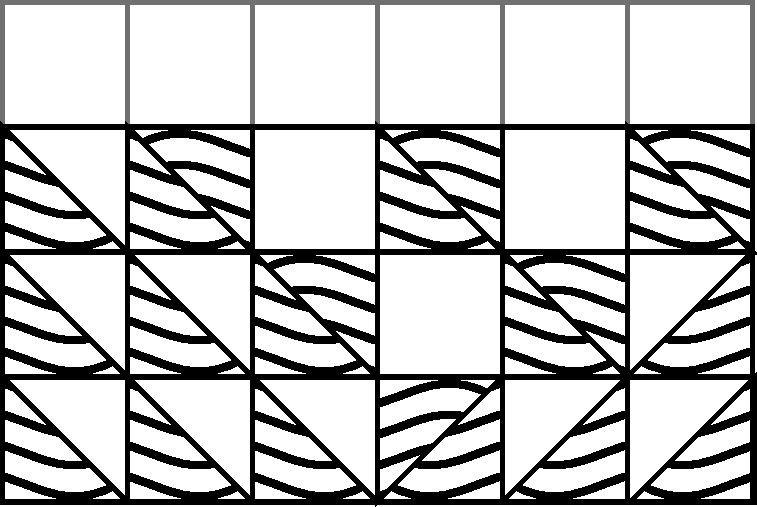
\includegraphics[width=.4\linewidth]{1.pdf}
				\end{center}
			\end{figure}
		
			After proving this result by induction, we get the desired answer:
			\[1+2+3\dots +49+49\dots + 2+1\]\hfill \qed
		\end{solution}
		
		
		When dealing with configurations like this, it is a good idea to think about how they could've been built. So it's useful to introduce ``time'' and gives us a way to progress algorithmically 
		
		\begin{example}(USAMO 1999 P1)
			Some checkers placed on an $ n \times n $ checkerboard satisfy the following conditions:
			
			\vspace{-1em} 
			
			\begin{enumerate}
				
				\item  every square that does not contain a checker shares a side with one that does;
				
				\item  given any pair of squares that contain checkers, there is a sequence of squares containing checkers, starting and ending with the given squares, such that every two consecutive squares of the sequence share a side.
			\end{enumerate}
			\vspace{-1em} 
			Prove that at least $ (n^{2}-2)/3 $ checkers have been placed on the board.
		\end{example}
	
		\begin{solution}
			The configuration is ``just there'', isn't it just too random? Let's try to see how it came to exist. (since we can't figure the fundamental question ``why anything exists'', we fool ourselves by trying to find meaning in meaningless board games, nice)
			
			So we have an empty board. We put checkers on it one by one. Call the squares that have a checker on itself or on one of its neighboring squares ``on''. We first put a checker on any square, and in the subsequent moves, we put a checker on a square, that is adjacent to a square already containing a checker. Since in the final configuration, all the squares that have a checker on them are connected, we can construct any configurations in this way.
			
			Now we count how many ``on'' squares we can make in each step. Since in the final state, we need $ n^2 $ ``on'' squares. In the first move, at most $ 5 $ squares are turning on. Then any move can turn at most $ 3 $ squares on (the square itself was already on, and one of its neighbors was on too).
			
			So if there are $ k $ squares on the board at the end, $ 5+3(k-1) \ge n^2 $ i.e. $ k\ge \dfrac{n^2-2}{3} $
		\end{solution}
		
		
		
		\subsection{Problems}
		
			The following problems use this basic strategy: start simple, focus on specific parts of the problem. They are in varying order of difficulty, so try them all.
		
			\begin{problem}(All-Russia 2018 Grade 9 P5)
				On the circle, 99 points are marked, dividing this circle into 99 equal arcs. Petya and Vasya play the game, taking turns. Petya goes first; on his first move, he takes a point and paints it red or blue. Then each player can paint on his own turn, in red or blue, any uncolored marked point adjacent to the already painted ones. Vasya wins, if after painting all points there is an equilateral triangle, all three vertices of which are colored in the same color. Could Petya prevent him?
			\end{problem}
		
			\begin{problem}(Indian Postal Coaching 2011)
				Consider $ 2011^2 $ points arranged in the form of a $ 2011 \times 2011 $ grid. What is the maximum number of points that can be chosen among them so that no four of them form the vertices's of either an isosceles trapezium or a rectangle whose parallel sides are parallel to the grid lines?
			\end{problem}
		
			\begin{problem}(Polish OI)
				Given $ n $ jobs, indexed from $ 1, 2\dots n $. Given two sequences of reals numbers, $ \{a_i\}^n_{i=1}, \{b_i\}^n_{i=1} $ where, $ 0 \leq a_i, b_i \leq 1 $. If job $ i $ starts at time $ t $ , then the job takes $ h_i(t) = a_it+b_i $ time to finish. Order the jobs in a way such that the total time taken by all of the jobs is the minimum.
			\end{problem}
		
			\begin{problem}
				A robot has $ n $ modes, and programmed as such: in mode $ i $ the robot will go at a speed of $ i \text{ms}^{-1} $ for $ i $ seconds. At the beginning of its journey, you have to give it a permutation of $ \{1, 2, \dots n \} $. What is the maximum distance you can make the robot go?
			\end{problem}
		
			\begin{problem}(ARO 2008 P9.5)
				The distance between two cells of an infinite chessboard is defined as the minimum number to moves needed for a king to move from one to the other. On the board are chosen three cells on pairwise distances equal to $ 100 $. How many cells are there that are at the distance $ 50 $ from each of the three cells?
			\end{problem}
		
			\begin{problem}(Brazilian Olympic Revenge 2014)
				Let $ n $ a positive integer. In a $ 2n\times 2n $ board, $ 1\times n $ and $ n\times 1 $ pieces are arranged without overlap. Call an arrangement maximal if it is impossible to put a new piece in the board without overlapping the previous ones. Find the least $ k $ such that there is a maximal arrangement that uses $ k $ pieces.
			\end{problem}
	
			\begin{problem}(ISL 2008 C1)
				In the plane we consider rectangles whose sides are parallel to the coordinate axes and have positive length. Such a rectangle will be called a box. Two boxes intersect if they have a common point in their interior or on their boundary. Find the largest $ n $ for which there exist $ n $ boxes $ B_1, B_2\dots B_n $ such that $ B_i $ and $ B_j $ intersect if and only if $ i \not\equiv j\pm 1\ (\bmod\ n) $.
			\end{problem}
	
	\section{Sherlock Holmes takes it home}	
	
	The old saying from The Holy Art And Craft Of Problem Solving: ``Get your hands dirty'' is the best advice ever. 
	
	
	\section{g0riber b0ndhu INDUCTION}
	
		This is everyone's favorite technique: induction. Since we cannot magically summon up a super solution, we start with smaller cases, check if we can somehow connect $ P(n) $ with $ P(n+1) $.
		
		We all know binary search, where we search by halving the search set on every step. This is a form of Divide and Conqure: when you don't have the power to exert dominance over a whole nation, divide it into small sections, ez. 
		
		Some general advice:
			
			\begin{enumerate}
				\itemsep0em
				\item In tougher problems, don't expect the induction to be very straightforward. You'll need more than that.
				\item In graph theory problems, removing one vertex or edge is most of the time the thing you need to do. But sometimes removing more than one vertice might be better.
				\item Always start with the strong induction hypothesis. More tools to play with.
				\item A lot of times, induction won't do you any good. But trying out induction is always one of the first few things one should do.
			\end{enumerate}
		
		Nothing new to introduce problem solving using induction, so let's jump right into the problems.
		
		
		
		\begin{problem}(All Russia 2017 9.1)
			In a country some cities are connected by oneway flights (There are no more then one flight between two cities). City $ A $ called "available" for city $ B $ , if there is flight from $ B $ to $ A $ , maybe with some transfers. It is known, that for every 2 cities $ P $ and $ Q $ exist city $ R $ , such that $ P $ and $ Q $ are available from $ R $. Prove, that exist city $ A $ , such that every city is available for $ A $.
		\end{problem}
	
		\begin{problem}(ARO 2013 P9.4)
			$ N $ lines lie on a plane, no two of which are parallel and no three of which are concurrent. Prove that there exists a non-self-intersecting broken line $ A_1A_2A_3\dots A_N $ with $ N $ parts, such that on each of the $ N $ lines lies exactly one of the $ N $ segments of the line.
		\end{problem}
	
		\begin{problem}(ISL 2010 C2)
			On some planet, there are $2^N$ countries $(N \geq 4).$ Each country has a flag $N$ units wide and one unit high composed of $N$ fields of size $1 \times 1,$ each field being either yellow or blue. No two countries have the same flag. We say that a set of $N$ flags is diverse if these flags can be arranged into an $N \times N$ square so that all $N$ fields on its main diagonal will have the same color. Determine the smallest positive integer $M$ such that among any $M$ distinct flags, there exist $N$ flags forming a diverse set.
		\end{problem}
		
		\begin{problem}(ISL 2016 C6)
			There are $ n \geq 3 $ islands in a city. Initially, the ferry company offers some routes between some pairs of islands so that it is impossible to divide the islands into two groups such that no two islands in different groups are connected by a ferry route.
			
			After each year, the ferry company will close a ferry route between some two islands $ X $ and $ Y $. At the same time, in order to maintain its service, the company will open new routes according to the following rule: for any island which is connected to a ferry route to exactly one of $ X $ and $ Y $, a new route between this island and the other of $ X $ and $ Y $ is added.
			
			Suppose at any moment, if we partition all islands into two nonempty groups in any way, then it is known that the ferry company will close a certain route connecting two islands from the two groups after some years. Prove that after some years there will be an island which is connected to all other islands by ferry routes.
		\end{problem}
		
		\begin{problem}(ISL 2005 C1)
			A house has an even number of lamps distributed among its rooms in such a way that there are at least three lamps in every room. Each lamp shares a switch with exactly one other lamp, not necessarily from the same room. Each change in the switch shared by two lamps changes their states simultaneously. Prove that for every initial state of the lamps there exists a sequence of changes in some of the switches at the end of which each room contains lamps which are on as well as lamps which are off.
		\end{problem}
	
		\begin{problem}(USAMO 2005 P1)
			Determine all composite positive integers $n$ for which it is possible to arrange all divisors of $n$ that are greater than $ 1 $ in a circle so that no two adjacent divisors are relatively prime.
		\end{problem}
	
		\begin{problem}
			Let $ S $ be a set with $ n $ elements, and let $ F $ be a family of subsets of S such that for any pair $ A, B $ in $ F $, $ A \cap B \not= \varnothing $. Then $ |F| \leq 2^{n-1} $.\footnote{This is actually an useful lemma.}
		\end{problem}
		
		\begin{problem}
			Let $ S $ be a set with $ n $ elements, and let $ F $ be a family of subsets of $ S $ such that for any pair $ A, B $ in $ F $, $ S $ is not contained by $ A \cup B $. Then $ |F| \leq 2^{n-1} $.\footnote{This one too.}
		\end{problem}
		
		\begin{problem}(USAMO 2005 P5)
			A mathematical frog jumps along the number line. The frog starts at $1$, and jumps according to the following rule: if the frog is at integer $n$, then it can jump either to $n+1$ or to $n + 2^{m_n+1}$ where $2^{m_n}$ is the largest power of $2$ that is a factor of $n$. Show that if $k \geq 2$ is a positive integer and $i$ is a nonnegative integer, then the minimum number of jumps needed to reach $2^ik$ is greater than the minimum number of jumps needed to reach $2^i.$
		\end{problem}
	
		\begin{problem}(ISL 2015 C1)
			In Lineland there are $n\geq1$ towns, arranged along a road running from left to right. Each town has a left bulldozer (put to the left of the town and facing left) and a right bulldozer (put to the right of the town and facing right). The sizes of the $2n$ bulldozers are distinct. Every time when a left and right bulldozer confront each other, the larger bulldozer pushes the smaller one off the road. On the other hand, bulldozers are quite unprotected at their rears; so, if a bulldozer reaches the rear-end of another one, the first one pushes the second one off the road, regardless of their sizes.
			
			Let $A$ and $B$ be two towns, with $B$ to the right of $A$. We say that town $A$ can sweep town $B$ away if the right bulldozer of $A$ can move over to $B$ pushing off all bulldozers it meets. Similarly town $B$ can sweep town $A$ away if the left bulldozer of $B$ can move over to $A$ pushing off all bulldozers of all towns on its way.
			
			Prove that there is exactly one town that cannot be swept away by any other one.
		\end{problem}
		
		\begin{problem}(ARO 2014 P9.3)
			In a convex $ n $ -gon, several diagonals are drawn. Among these diagonals, a diagonal is called good if it intersects exactly one other diagonal drawn (in the interior of the $ n $ -gon). Find the maximum number of good diagonals.
		\end{problem}
	
		\begin{problem}(ISL 2013 C2)
			A configuration of $ 4027 $ points in the plane is called Colombian if it consists of $ 2013 $ red points and $ 2014 $ blue points, and no three of the points of the configuration are collinear. By drawing some lines, the plane is divided into several regions. An arrangement of lines is good for a Colombian configuration if the following two conditions are satisfied:
			\vspace{-1em}			
			\begin{enumerate}
				\item No line passes through any point of the configuration.
				\item No region contains points of both colors.
			\end{enumerate}
			\vspace{-1em}
			Find the least value of $ k $ such that for any Colombian configuration of $ 4027 $ points, there is a good arrangement of $ k $ lines.
		\end{problem}
		
		Sometimes there are traps like this, which motivates you to try induction, but doesn't yeild any good results. But still, trying out induction gets you closer to the correct solution. 
	
		\begin{problem}
			There are $ 100 $ points on the plane. You have to cover them with discs, so that any two disks are at a distance of $ 1 $. Prove that you can do this in such a way that the total diameter of the disks is $ < 100 $
		\end{problem}
		
	
	\section{Random stuffs because you have to}
	
	\section{More random stuffs, because why not}
	
		\begin{problem}(ISL 1991 P10)
			Suppose $ \,G\,$ is a connected graph with $ \,k\,$ edges. Prove that it is possible to label the edges $ 1,2,\ldots ,k\,$ in such a way that at each vertex which belongs to two or more edges, the greatest common divisor of the integers labeling those edges is equal to $ 1 $.
		\end{problem}
	
	\section{send it to graph}
	
	\begin{problem}
		Given $ 2n+1 $ irrational numbers, prove that one can pick $ n $ from them s.t. no two of the choosen $ n $ sum up to a rational number.
	\end{problem}

\end{document}